\documentclass[12pt]{article}



\usepackage[T1]{fontenc}
\usepackage{amsfonts, amsmath, amssymb}
\usepackage{multirow}
\usepackage{epsfig}
\usepackage{subcaption}
\usepackage{graphicx}
% \usepackage{xurl}
\usepackage{hyperref}
\usepackage{parskip}
\usepackage{booktabs}
\usepackage{longtable}
\usepackage[utf8]{inputenc}
\usepackage[english]{babel}
% \usepackage[document]{ragged2e}
\usepackage{verbatim, rotating, paralist}
\usepackage{enumerate}

\usepackage{natbib}
\usepackage{array}

\usepackage{pdfsync}
\usepackage{latexsym}
\usepackage{amsthm}
% \usepackage{mathabx}

\usepackage{stmaryrd}
\usepackage{mathrsfs}
% \usepackage{dsfont}
\usepackage{fancyhdr}
\usepackage{color}

\usepackage{parskip}
% \usepackage{anysize, indentfirst, setspace}
% \usepackage[right=1.75cm, left=1.75cm, top=3cm, bottom=3cm]{geometry}
\usepackage{appendix}

\usepackage{enumitem}
\setlist{nosep}

\renewcommand{\topfraction}{.85}
\renewcommand{\bottomfraction}{.7}
\renewcommand{\textfraction}{.15}
\renewcommand{\floatpagefraction}{.66}
\renewcommand{\dbltopfraction}{.66}
\renewcommand{\dblfloatpagefraction}{.66}




% \pagestyle{fancyplain}
% \rhead{\hfill \small \emph{MIDS NUMBER -- Fall 2019}}
\cfoot{}

% \renewcommand{\headrulewidth}{0pt}


\title{Backwards Design Template}

%-------------------------- BEGIN DOCUMENT ----------------------------------%
\begin{document}
\maketitle

\section{Topic}
\emph{What problem are you (or your stakeholder) trying to address?}

The overall problem we are trying to address is the opioid epidemic in the 
United States.
\vspace*{2cm}\\


\section{Project Question}
\emph{What specific question are you seeking to answer with this project?}

How does state-level opioid prescribing legislation affect opioid-related 
overdose death rates and opioid prescription rates in the United States?
\vspace*{2cm}\\


\section{Project Hypothesis}
\emph{What is your hypothesized answer to your question?}

$H_0$ \emph{(Null Hypothesis)}: State-level opioid prescribing legislation did 
not affect opioid prescription rates or opioid-related overdose death rates.

$H_A$ \emph{(Alternative Hypothesis)}: State-level opioid prescribing 
legislation caused a decrease in at least one of these outcomes. 

\emph{Our guess}: We expect opioid prescription rates to decrease following the 
implementation of the legislation, while the direction of the change in opioid-
related overdose death rates remains uncertain.
\vspace*{2cm}\\

\section{Model Results}
\emph{One of the hardest parts of developing a good data science project is 
developing a question that is actually answerable. Perhaps the best way to 
figure out if your question is answerable is to see if you can imagine what an 
answer to your question would look like. Below, draw the graph, regression 
table, etc. that you would consider to be an answer to your question. Then draw 
it again, so you have a model result for if your hypothesized answer is true, 
and a model result for if your hypothesized answer is false. (If the answer to 
your question is continuous, not discrete (e.g. ``what is the level of 
inequality in the United States?''), draw it for high values (high inequality) 
and low values (low inequality)).}

\begin{minipage}{0.5\textwidth}
\centering
\textbf{Result if your hypothesis is true}
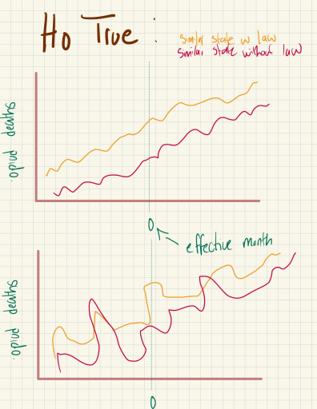
\includegraphics[width=0.9\linewidth]{H0_graphical_example.png}
\end{minipage}%
\begin{minipage}{0.5\textwidth}
\centering
\textbf{Result if your hypothesis is false}
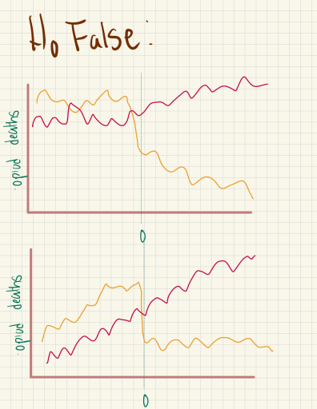
\includegraphics[width=0.9\linewidth]{HA_graphical_example.png}
\end{minipage}
\vspace*{2cm}\\
\section{Final Variables Required}

\emph{Now that you've specified what an answer to your question looks like, what 
data do you need to generate that answer?}

\emph{You don't have to know the exact variable and dataset (``I need 
\texttt{ANNPOP2008} from the NHGIS 2019 census 1\% sample release''), but you 
should be specific enough that all properties that are critical to your analysis 
are fully specified (e.g., I need individual-level annual income data for a 
nationally representative sample of all working US citizens).}

\emph{Basically, this should be a list of all the variables (not in terms of 
specific variable names, but the substantive content of each variable) that you 
need in hand to do the analysis proposed above \textbf{and} an explanation of 
the population represented in that data (i.e., what is represented by each row 
of your data, and what is the group of entities included in the data). In other 
words, what variables would be the direct inputs into the plots/model results 
described above?}

Variables needed in final dataset:
\begin{itemize}
    \item County
    \item State
    \item Year
    \item Pre/Post legislation indicator (0 = pre-legislation, 1 = post-
    legislation)
    \item County Population
    \item Drug statistics:
    \begin{itemize}
        \item Opioid-related overdose death count
        \item Opioid prescription quantity prescribed
        \begin{itemize}
            \item This is based on the quantity (count/weight/volume) shipped 
            into the county
        \end{itemize}
    \end{itemize}
    \item County-level covariates:
    \begin{itemize}
        \item Median household income
        \item Unemployment rate
        \item Cost of living (defined as Personal Consumption Expenditures)
        \item Race proportions
        \end{itemize}
\end{itemize}

All values are per county per year.\\
Generally, we can assume that shipment quantities relate to what is being 
prescribed\\
Death rate = county opiod deaths / county population


\pagebreak
\section{Data Sources}

\emph{Given the variables you need for your analysis, what actual data sources 
do you think will have the data you need?}

\emph{In specifying the datasets you need, if you list more than one 
\textbf{also} indicate how you think you can relate these datasets (i.e. if 
you're gonna merge datasets, what variables do you think those datasets will 
provide that will allow you merge them? There's no use saying ``I'll merge this 
political survey with medical records of who has received bad care'' if the 
political survey doesn't provide identifying information you can use to link 
survey respondents to medical records, even if you have both the survey and 
medical records!)}

\emph{If you are familiar with \href{https://www.visual-paradigm.com/guide/data-modeling/what-is-entity-relationship-diagram/}{\underline{Entity Relational Diagrams}} for databases, something similar is a great way of diagramming how you expect datasets you plan to use will relate to one another.}

\begin{tabular}{>{\raggedright\arraybackslash}p{0.28\textwidth} | >{\raggedright\arraybackslash}p{0.36\textwidth} | >{\raggedright\arraybackslash}p{0.28\textwidth}}
    \textbf{Dataset Name}& \textbf{Variables we can use} & \textbf{Link}  \\ \hline
    NBER Census CBSA–FIPS County Crosswalk & County FIPS, State FIPS, CBSA code, County name, CBSA name & \url{https://www.nber.org/research/data/census-core-based-statistical-area-cbsa-federal-information-processing-series-fips-county-crosswalk} \\ \hline
    BEA Regional Price Parities (RPP) & Regional Price Parity (RPP), Year, State/Metropolitan Area, Cost of Living Index & \url{https://www.bea.gov/data/prices-inflation/regional-price-parities-state-and-metro-area} \\ \hline
    BLS Local Area Unemployment Statistics (LAUS) & County FIPS, Year, Unemployment Rate, Employment, Labor Force & \url{https://www.bls.gov/lau/tables.htm} \\ \hline
    U.S. Census Bureau American Community Survey (ACS) 5-Year Estimates & County FIPS, Year, Race, Ethnicity, Median Household Income, Poverty Rate & \url{https://www.census.gov/data/developers/data-sets/acs-5year.html}
\end{tabular}
\vspace*{2cm}\\

\section{Division of Labor}

\emph{Now that you have identified what needs to be done, how do you plan to 
divide those tasks among team members?}

\subsection{Tiye}
\begin{itemize}
    \item Find data sources
    \item Clean BLS LAUS file
    \item Plot figures
\end{itemize}

\subsection{Royce}
\begin{itemize}
    \item Clean 12 GB file
    \item Clean BEA RPP file
    \item Merge files
\end{itemize}

\subsection{Laura}
\begin{itemize}
    \item Clean ACS file
    \item Clean NBER file
    \item Design regression models
\end{itemize}

\end{document}
